 \documentclass[aspectratio=169,11pt]{beamer}

% Theme and colours
\usetheme{Madrid}
\usecolortheme{default}
\definecolor{oruBlue}{RGB}{0,63,114}
\definecolor{oruGray}{RGB}{100,100,100}
\setbeamercolor{structure}{fg=oruBlue}
\setbeamercolor{frametitle}{bg=oruBlue,fg=white}
\setbeamercolor{title}{bg=oruBlue,fg=white}
\setbeamercolor{block title}{bg=oruBlue,fg=white}
\setbeamercolor{item}{fg=oruBlue}
\setbeamercolor{footline}{fg=oruGray}
\setbeamertemplate{blocks}[rounded][shadow=false]                              


% Packages
\usepackage[utf8]{inputenc}
\usepackage[T1]{fontenc}
\usepackage{graphicx}
\usepackage{booktabs}
\usepackage{amsmath}
\usepackage{tikz}
\usepackage{hyperref}
\usepackage{appendixnumberbeamer}

% Suppress navigation symbols
\setbeamertemplate{navigation symbols}{}

% Footline with short info
\setbeamertemplate{footline}{%
  \leavevmode%
  \hbox{%
    \begin{beamercolorbox}[wd=.4\paperwidth,ht=2.5ex,dp=1ex,left]{footline}%
      \hspace*{2mm}\footnotesize 
    \end{beamercolorbox}%
    \begin{beamercolorbox}[wd=.3\paperwidth,ht=2.5ex,dp=1ex,center]{footline}%
      \footnotesize 
    \end{beamercolorbox}%
    \begin{beamercolorbox}[wd=.3\paperwidth,ht=2.5ex,dp=1ex,right]{footline}%
      \footnotesize\insertframenumber{}/\inserttotalframenumber\hspace*{2mm}
    \end{beamercolorbox}}%
  \vskip0pt%
}


\setbeamertemplate{footline}{%
  \leavevmode%
  \hbox{%
    \begin{beamercolorbox}[wd=.4\paperwidth,ht=2.5ex,dp=1ex,left]{footline}%
      \hspace*{2mm}\footnotesize 
    \end{beamercolorbox}%
    \begin{beamercolorbox}[wd=.3\paperwidth,ht=2.5ex,dp=1ex,center]{footline}%
      \footnotesize 
    \end{beamercolorbox}%
    \begin{beamercolorbox}[wd=.3\paperwidth,ht=2.5ex,dp=1ex,right]{footline}%
      \footnotesize\insertframenumber{}/\inserttotalframenumber\hspace*{2mm}
    \end{beamercolorbox}}%
  \vskip0pt%
}

% Figure path
\graphicspath{{../figures/}{./}}

% Meta
\title[Canaries in the Coal Mine]{Same Storm, Different Boats:\\Generative AI and the Age Gradient in Hiring}
\author[Lodefalk]{Magnus Lodefalk\inst{1,2} \and Lydia Löthman\inst{1} \and Michael Koch\inst{3,4} \and Erik Engberg\inst{1,2}}
\institute[ORU]{\inst{1}Örebro University \inst{2}RATIO Institute \inst{3}Aarhus University \inst{4}Kiel Institute}
\date{28 Maj 2026}



\begin{document}

% ============================================================
% TITLE SLIDE
% ============================================================
\begin{frame}[plain]
\titlepage
\vspace{-6mm}
\begin{center}
\raisebox{-0.5\height}{
\includegraphics[height=0.7cm]{orebro_logo.png}}\hspace{6mm}%
\raisebox{-0.5\height}{
\includegraphics[height=0.55cm]{ratio_logo.png}}\hspace{6mm}%
\raisebox{-0.5\height}{
\includegraphics[height=0.6cm]{ai_econ_lab_logo.png}}\hspace{6mm}%
\raisebox{-0.5\height}{
\includegraphics[height=0.55cm]{aiscaf_logo.png}}\hspace{6mm}%
\raisebox{-0.5\height}{
\includegraphics[height=0.45cm]{wasphs_logo.png}}
\end{center}
\end{frame}


\begin{frame}{Från optimism till oro kring generativ AI}

\textbf{Tidiga studier präglades huvudsakligen av optimism}
\begin{itemize}
    \item Experimentella studier visade betydande produktivitetseffekter (Noy \& Zhang, 2023)
    \item Företag som tidigt implementerade AI-lösningar tenderade att expandera sin arbetsstyrka (Hellsten et al., 2025)
    \item Produktivitetsvinster förväntades öka efterfrågan på arbetskraft och samtidigt skapa nya arbetsuppgifter och yrkesroller
\end{itemize}

\vspace{3mm}

\textbf{Mot slutet av 2025 började dock bilden bli mer nyanserad}

\vspace{2mm}

\textbf{”Canaries in the Coal Mine” (Brynjolfsson et al., 2025)}
\begin{itemize}
    \item Analys av amerikansk sysselsättningsstatistik efter genombrottet för generativ AI och ChatGPT
    \item Fokus på AI-exponerade yrken där arbetsuppgifter i hög grad kan utföras eller stödjas av AI-verktyg
    \item Cirka 13-procentig relativ nedgång i sysselsättning för unga i AI-exponerade yrken
    \item Ingen motsvarande nedgång för äldre inom samma yrkeskategorier
\end{itemize}

\end{frame}


% ============================================================
% DATA
% ============================================================
\begin{frame}{Den stora frågan: Syns samma tendenser i Sverige?}

\begin{itemize}
    \item Genom att använda lönedata från SCB analyserar vi sysselsättningsutvecklingen i Sverige sedan lanseringen av ChatGPT 
\end{itemize}
\vspace{5mm}

\begin{center}
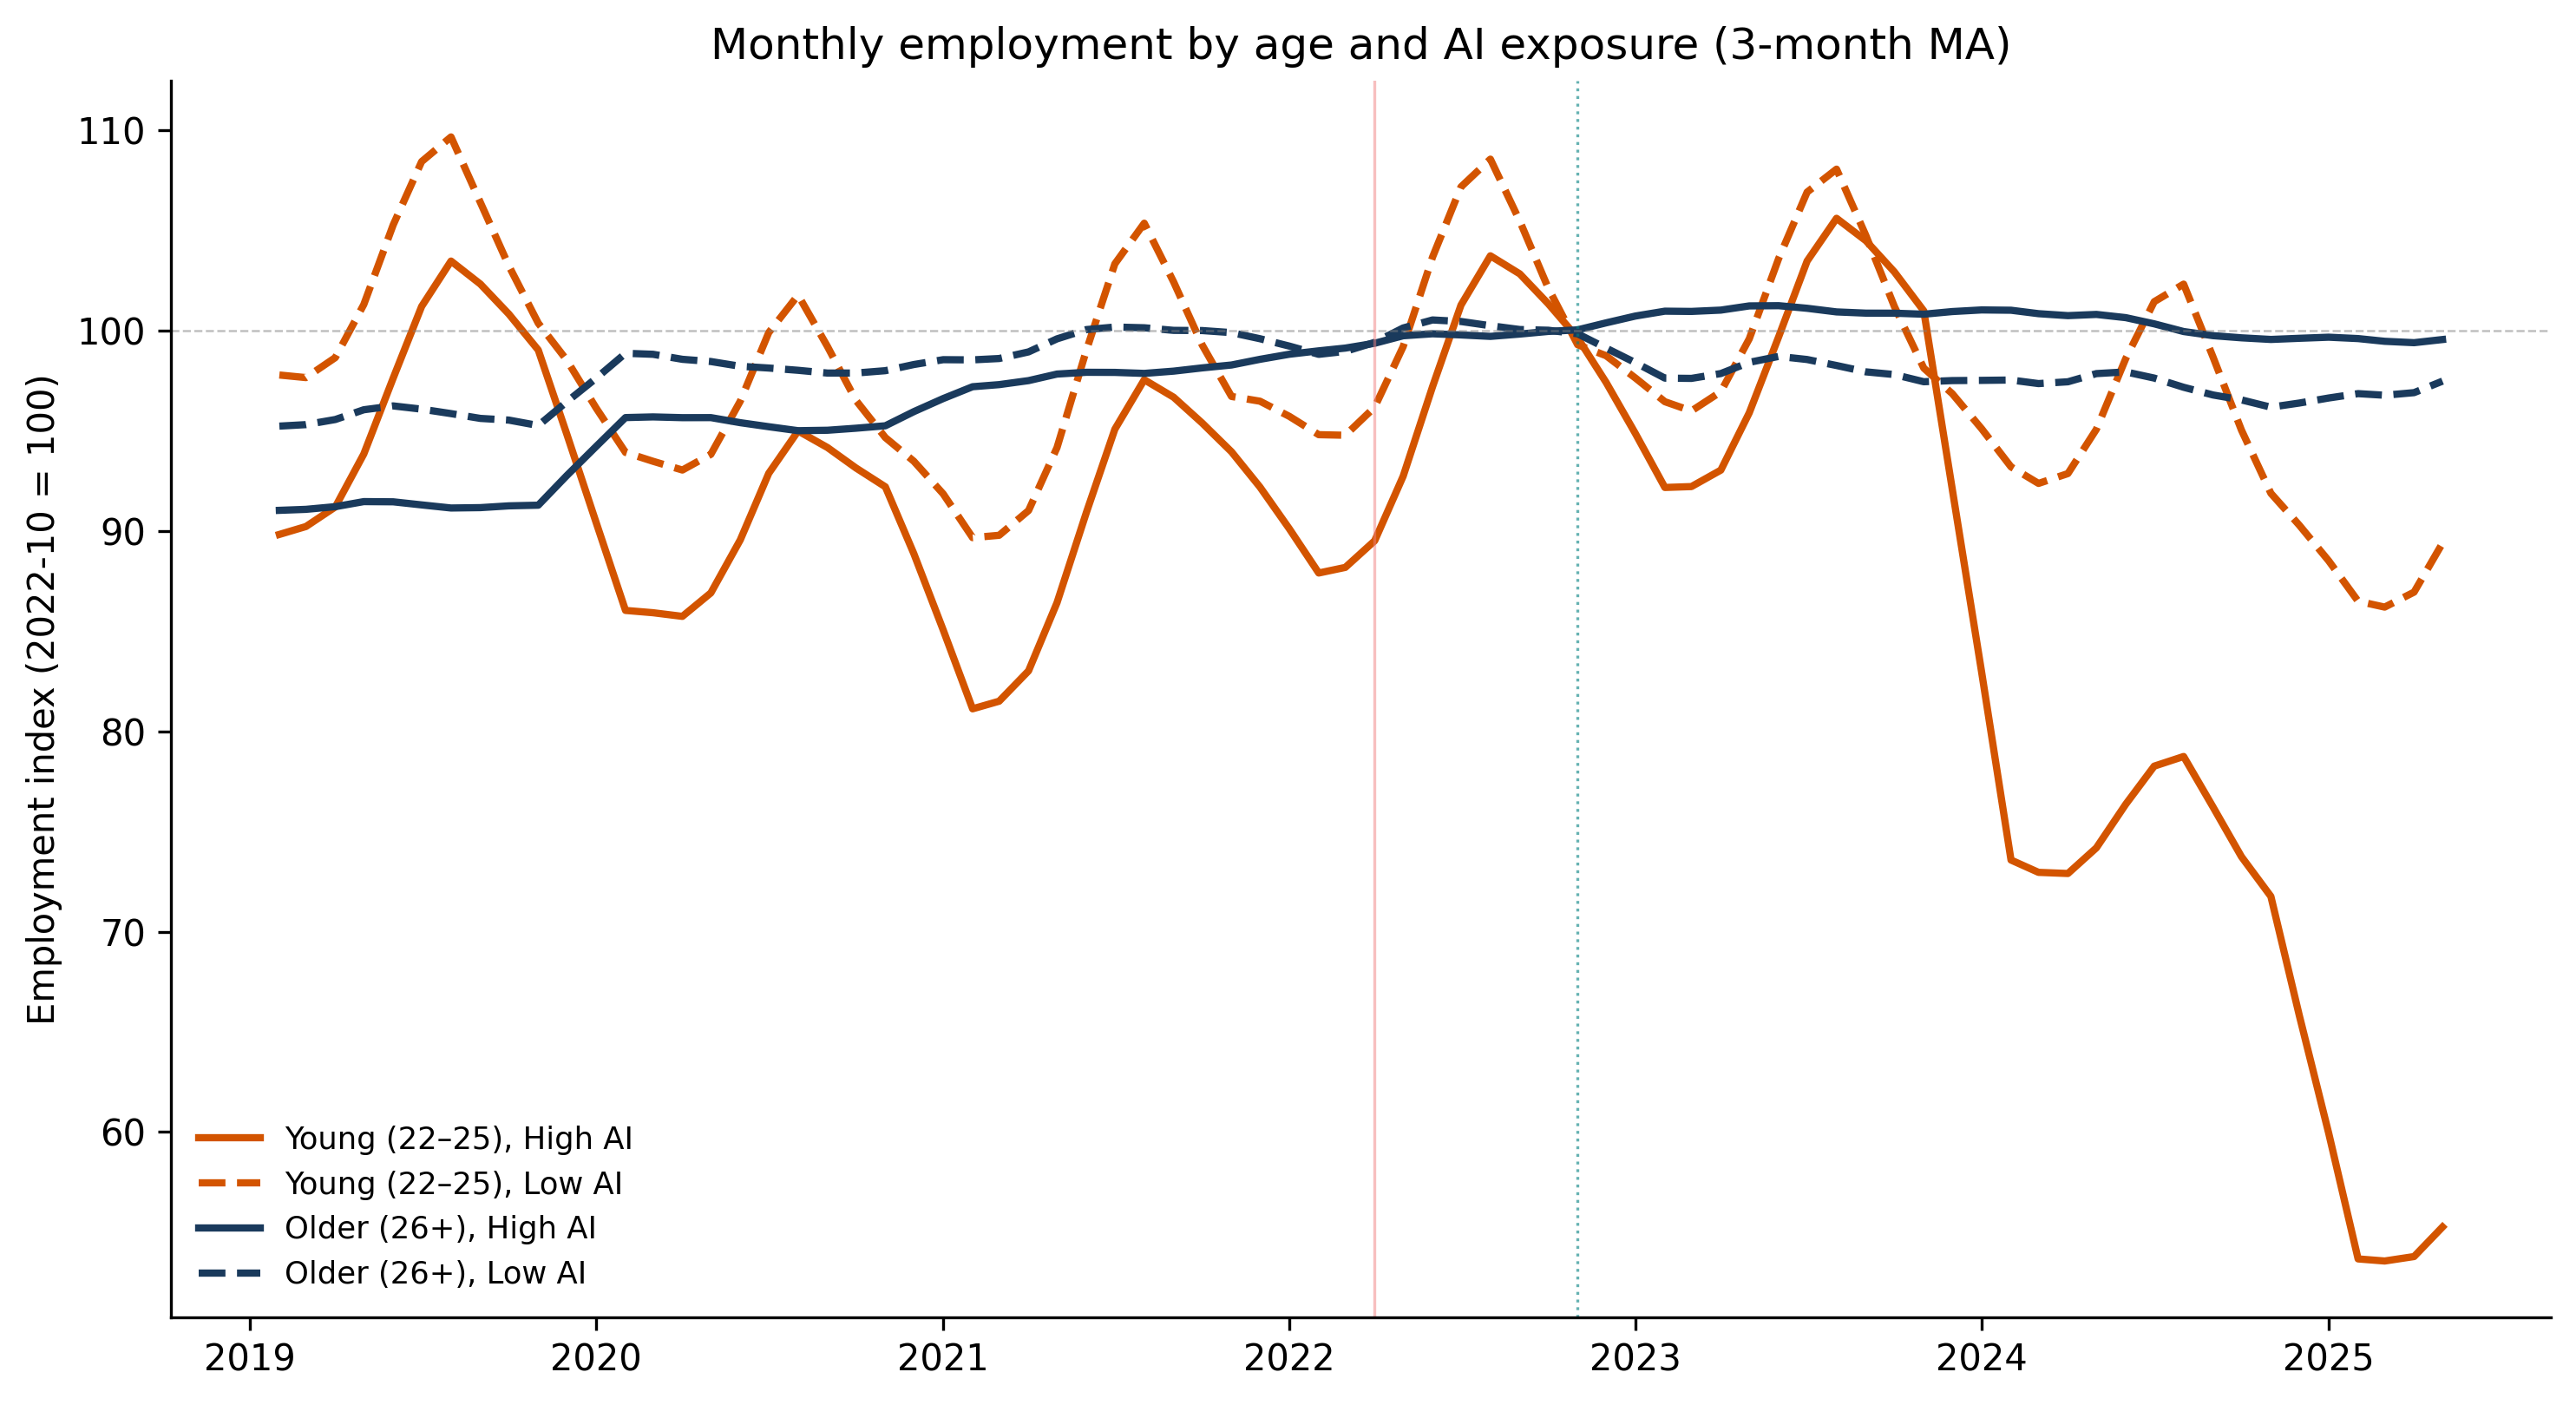
\includegraphics[width=0.6\textwidth]{fig2_mona_canaries_ma3.png}
\end{center}
\end{frame}


% ============================================================
% DAIOE: AI EXPOSURE MEASURE
% ============================================================
\begin{frame}{Vad innebär AI-exponering?}
\begin{columns}[T]
\begin{column}{0.55\textwidth}
\textbf{Dynamiskt AI-exponerings mått (DAIOE)} (Engberg et al.\ 2024)
\begin{enumerate}
  \begin{itemize}
    \item Utgår från ett antal färdigheter som AI kan utföra i varierande grad
    
    \item Matchar dessa färdigheter mot O*NET:s bedömningar av kognitiva arbetsuppgifter
    
    \item Aggregerar färdighetsmåtten till yrkesnivå
    
    \item Matchar därefter till svenska yrken med hjälp av SCB:s yrkesklassificering

    \item AI är framförallt duktig på \textit{rutinbaserade} och \textit{kognitiva} arbetsuppgifter som inte kräver sociala färdigheter
\end{itemize}
\end{enumerate}
\vspace{2mm}
\begin{itemize}
    \item Fångar vad AI teoretiskt sett \textit{kan} göra, inte faktiskt AI-adaptering
\end{itemize}
\end{column}
\begin{column}{0.42\textwidth}
\begin{block}{Högst exponering (Q4)}
\footnotesize
Kundtjänstpersonal, löneadministratörer, receptionists, mjukvaruutvecklare, revisorer, sekreterare
\end{block}
\vspace{2mm}
\begin{block}{Lägst exponering (Q1)}
\footnotesize
Byggarbetare, städare, sjukvårdspersonal, kockar, förskolelärare
\end{block}
\end{column}
\end{columns}
\hypertarget{main:daioe}{}
\end{frame}

% ============================================================
% RESULT: EVENT STUDY
% ============================================================
\begin{frame}{Accelrerande åldergradient}
\begin{columns}[c]
\begin{column}{0.48\textwidth}
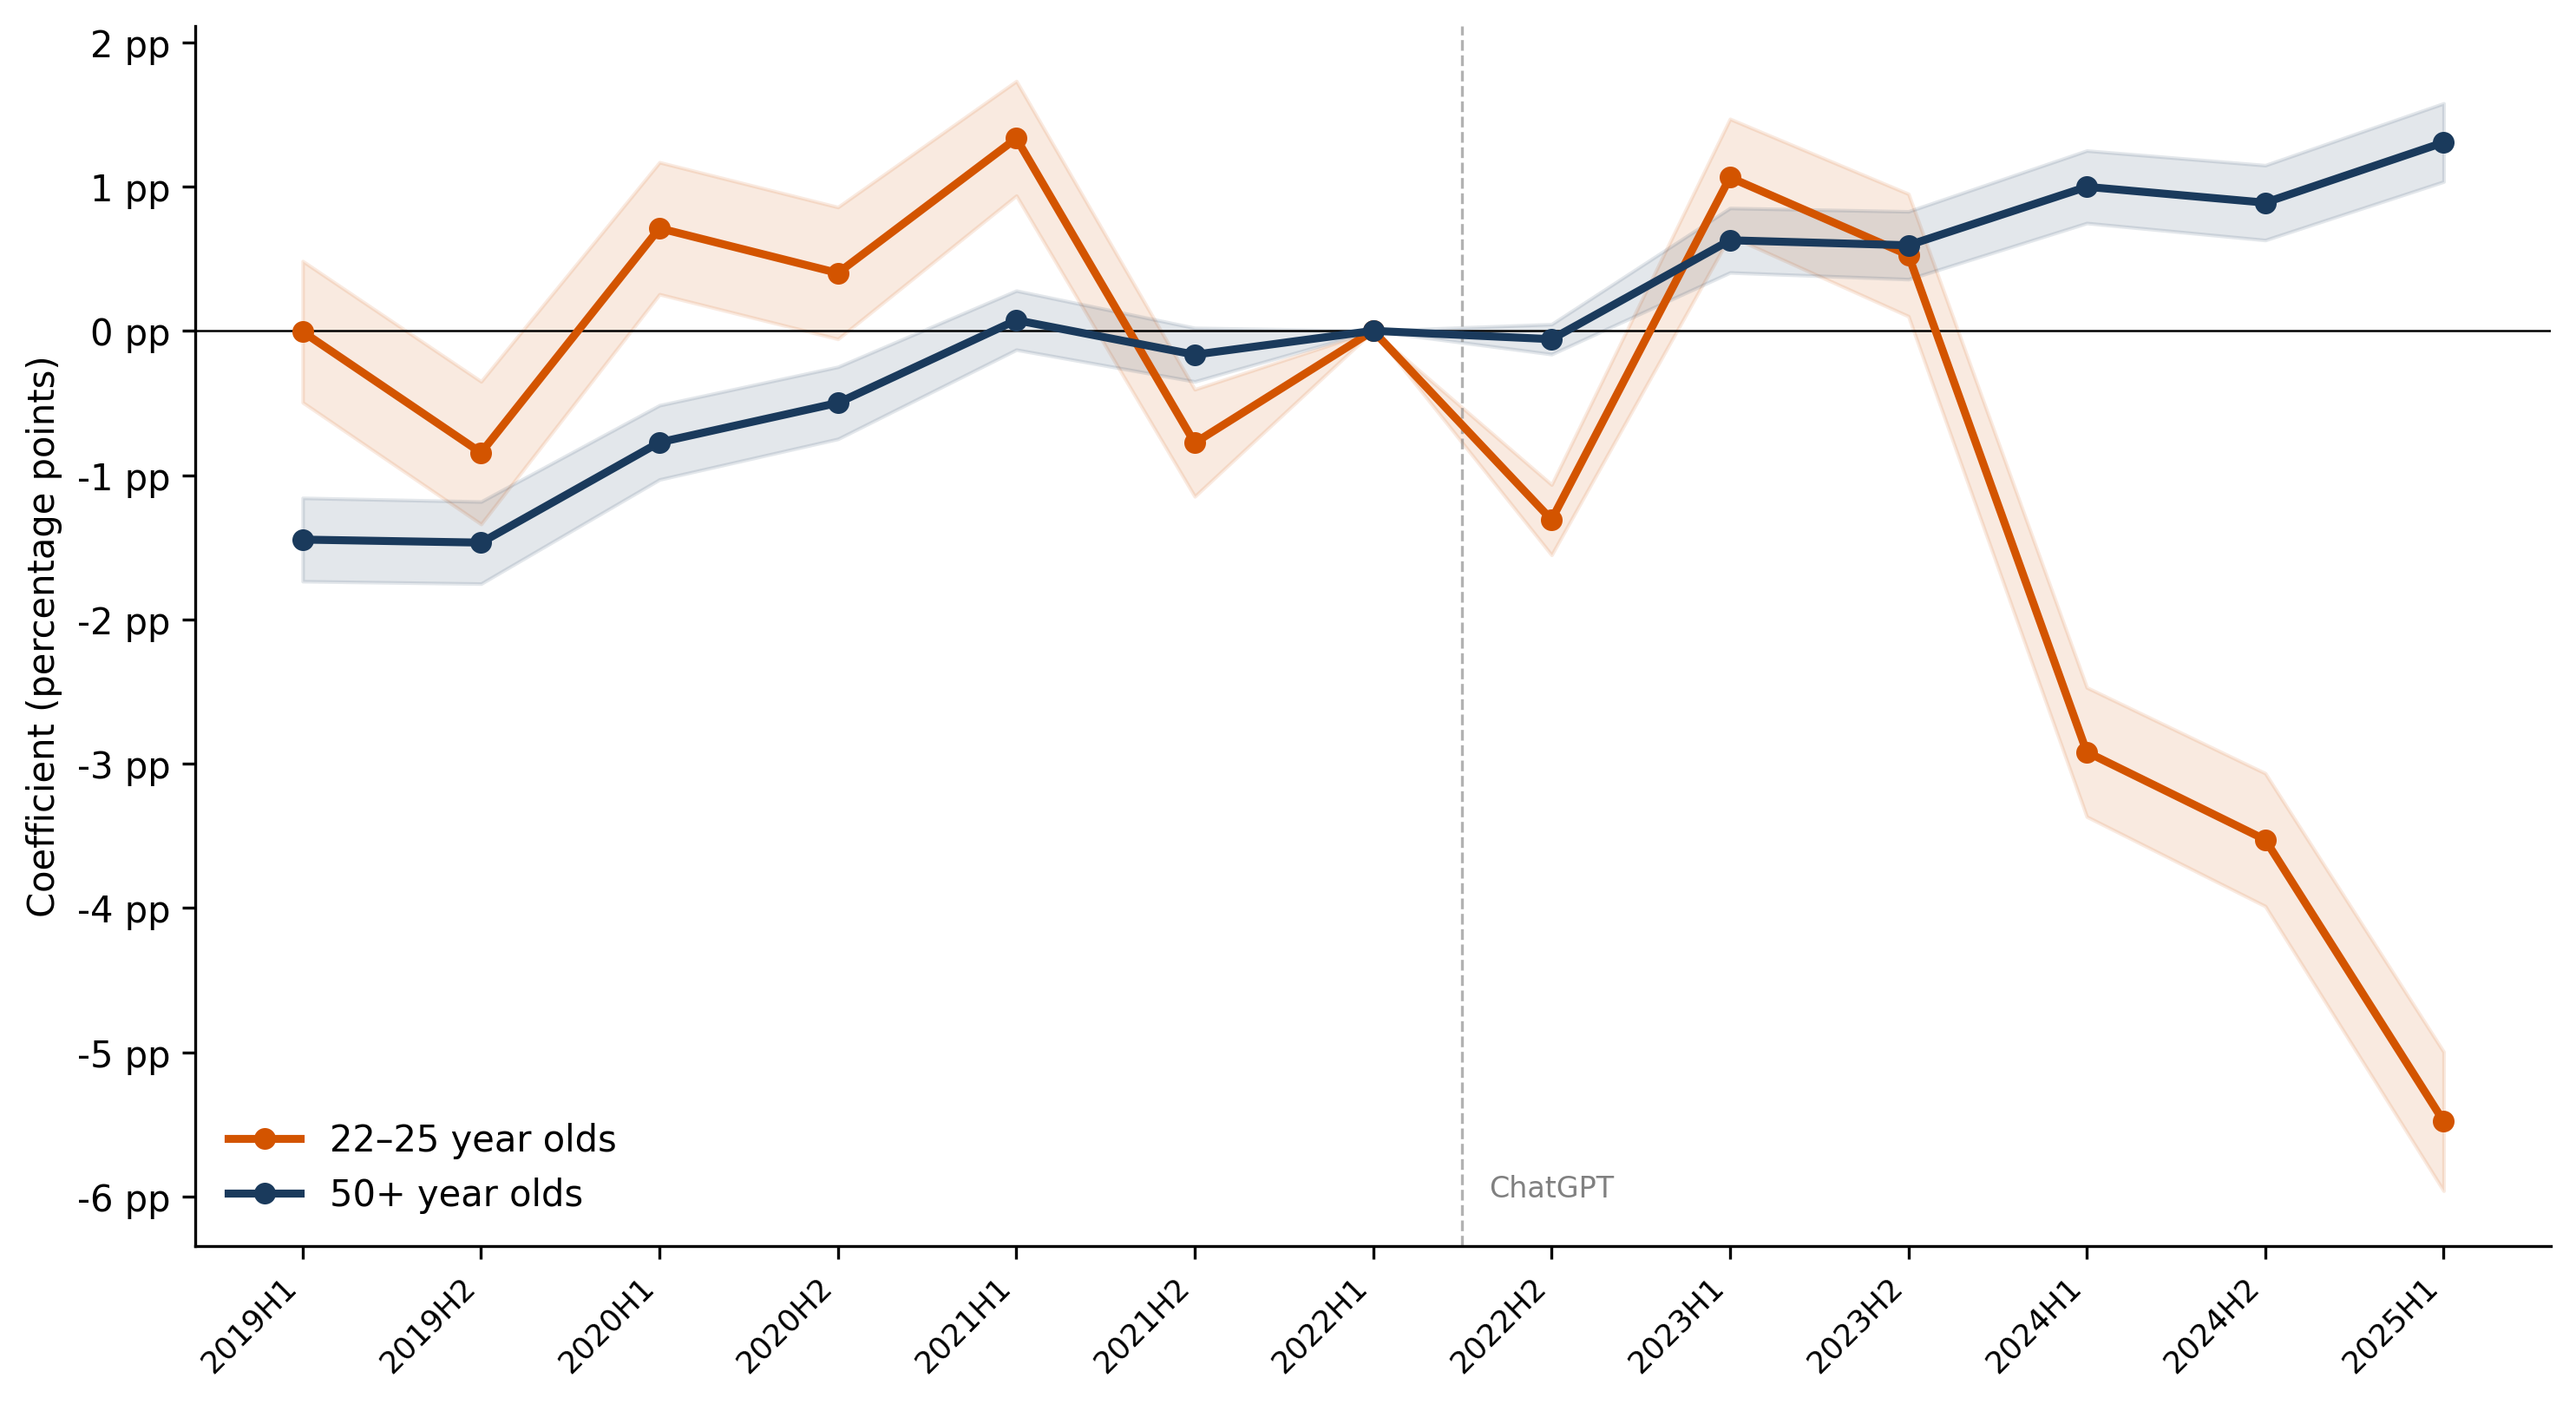
\includegraphics[width=\textwidth]{fig3_event_study_main.png}
\end{column}
\begin{column}{0.50\textwidth}
\textbf{Nyckeltal:}
\begin{itemize}
    \item 22--25 i de högst exponerade yrkena: $-5.5\%$ i början av 2025
    \item 26--30 i de högst exponerade yrkena: $-4.9\%$ i början av 2025
    \item 50+ i de högst exponerade yrkena: $+1.3\%$
\end{itemize}
\vspace{3mm}
\textbf{Färre unga nyanställs:}
\begin{itemize}
\begin{itemize}
    \item För 22–25 drivs nedgången främst av färre nyanställningar
    
    \item För 50+ ökar både nyanställningar och separationer, men nettoeffekten är positiv
\end{itemize}
\end{itemize}
\vspace{2mm}
\end{column}
\end{columns}
\end{frame}


\begin{frame}{Internationell jämförelse}

\small

\begin{table}[h]
\centering
\begin{tabular}{p{2.3cm} p{3.3cm} p{4.8cm}}
\hline
\textbf{Studie} & \textbf{Huvudresultat} & \textbf{Tolkning} \\
\hline

USA &
13\,\% nedgång i sysselsättning &
Liknande metod och samma övergripande mönster som i Sverige \\[2mm]

Sverige &
5.5\,\% nedgång i sysselsättning &
Negativa sysselsättningseffekter för unga i AI-exponerade yrken \\[2mm]

Danmark &
Inga tydliga löneeffekter &
Begränsad jämförbarhet på grund av skillnader i data och metod
 \\[2mm]

Finland &
Inga tydliga sysselsättningseffekter &
Skillnaden kvarstår trots metodologiska anpassningar mot deras ansats \\

\hline
\end{tabular}
\end{table}

\vspace{2mm}

\footnotesize
Möjliga förklaringar: institutionella skillnader och variation i AI-adoption.

\end{frame}


\section{Interpretation}


% ============================================================
% INTERPRETATION
% ============================================================
\begin{frame}{Tänkbar tolkning: den färdighetsbaserade modellen}
\begin{center}
\resizebox{0.8\textwidth}{!}{
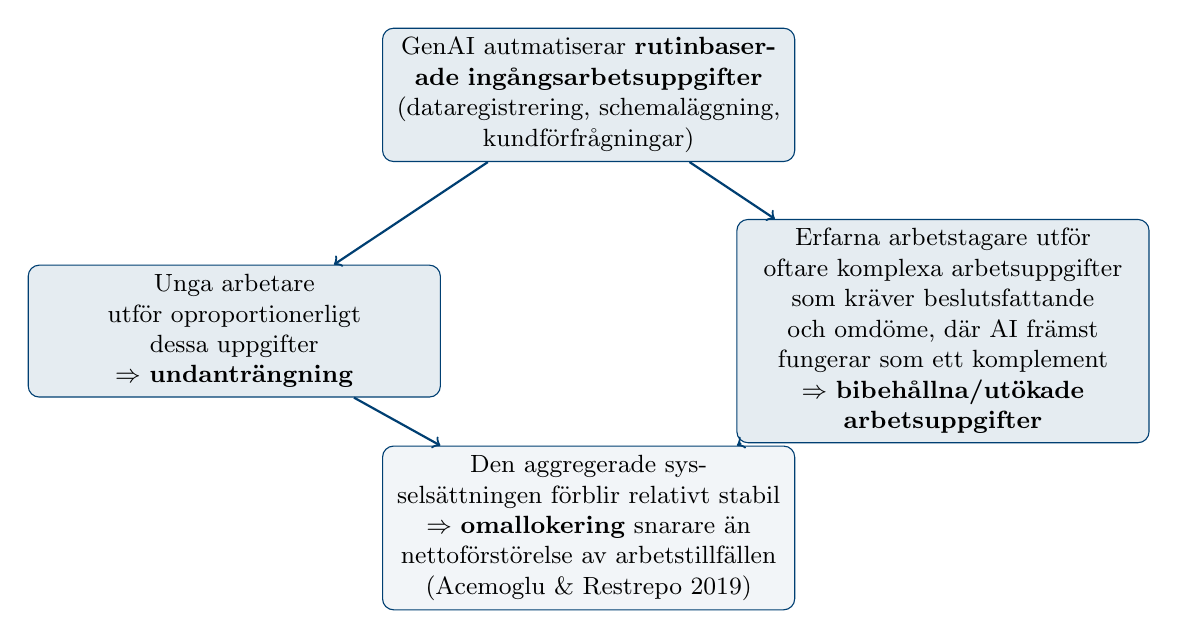
\begin{tikzpicture}[
    box/.style={rectangle, draw=oruBlue, fill=oruBlue!10, rounded corners, text width=5cm, minimum height=1.2cm, align=center, font=\small},
    arrow/.style={->, thick, oruBlue}
]
\node[box] (ai) at (0,3) {GenAI autmatiserar \textbf{rutinbaserade ingångsarbetsuppgifter}\\(dataregistrering, schemaläggning, kundförfrågningar)};
\node[box] (young) at (-4.5,0) {Unga arbetare\\utför oproportionerligt\\dessa uppgifter\\$\Rightarrow$ \textbf{undanträngning}};
\node[box] (old) at (4.5,0) {Erfarna arbetstagare utför oftare komplexa arbetsuppgifter som kräver beslutsfattande och omdöme, där AI främst fungerar som ett komplement $\Rightarrow$ \textbf{bibehållna/utökade arbetsuppgifter}};
\node[box, fill=oruBlue!5] (net) at (0,-2.5) {Den aggregerade sysselsättningen förblir relativt stabil\\$\Rightarrow$ \textbf{omallokering} snarare än nettoförstörelse av arbetstillfällen\\(Acemoglu \& Restrepo 2019)};
\draw[arrow] (ai) -- (young);
\draw[arrow] (ai) -- (old);
\draw[arrow] (young) -- (net);
\draw[arrow] (old) -- (net);
\end{tikzpicture}
}
\end{center}

\vspace{2mm}
{\footnotesize \textit{Svensk anställningsskyddslagstiftning skyddar dock seniora arbetstagare, vilket innebär att effekten inte fullt ut kan särskiljas från AI-komplementaritet.}}
\end{frame}



\section{Conclusion}

% ============================================================
% CONCLUSION AND POLICY
% ============================================================
\begin{frame}{Slutsatser}
\begin{columns}[T]

\begin{column}{0.48\textwidth}
\begin{itemize}
    \item Ingen tydlig nedgång i sysselsättningen på aggregerad nivå
    
    \item När sysselsättningen bryts ned efter ålder och yrkeskategori framträder tydliga skillnader
    
    \item Unga människor, särskilt unga kvinnor, verkar få allt svårare att etablera sig i AI-exponerade yrken
\end{itemize}
\end{column}

\begin{column}{0.48\textwidth}
\begin{itemize}
    
    \item Mer forskning krävs för att identifiera mekanismerna bakom resultaten och skillnader mellan länder
    
\end{itemize}
\end{column}

\end{columns}

\vfill

\centering
\large Tack! Frågor?

\vspace{2mm}

\normalsize lydia.lothman@oru.se

\end{frame}

\end{document}
